\documentclass[11pt,compress,t,notes=noshow, xcolor=table]{beamer}
\usepackage[]{graphicx}\usepackage[]{color}
% maxwidth is the original width if it is less than linewidth
% otherwise use linewidth (to make sure the graphics do not exceed the margin)
\makeatletter
\def\maxwidth{ %
  \ifdim\Gin@nat@width>\linewidth
    \linewidth
  \else
    \Gin@nat@width
  \fi
}
\makeatother

\newcommand{\citebutton}[2]{%
\beamergotobutton{\href{#2}{#1}}%
}

\newcommand{\blu}[1]{\textcolor{blue}{#1}}
\newcommand{\org}[1]{\textcolor{orange}{#1}}
\newcommand{\ques}{\textbf{\textcolor{red}{Question:  }}}
\newcommand{\questionssofar}{\begin{frame}\frametitle{Any questions?}\end{frame}}

\newcommand\warning{%
 \makebox[1.4em][c]{%
 \makebox[0pt][c]{\raisebox{.1em}{\scriptsize!}}%
 \makebox[0pt][c]{\color{red}\normalsize$\bigtriangleup$}}}%

\definecolor{fgcolor}{rgb}{0.345, 0.345, 0.345}
\newcommand{\hlnum}[1]{\textcolor[rgb]{0.686,0.059,0.569}{#1}}%
\newcommand{\hlstr}[1]{\textcolor[rgb]{0.192,0.494,0.8}{#1}}%
\newcommand{\hlcom}[1]{\textcolor[rgb]{0.678,0.584,0.686}{\textit{#1}}}%
\newcommand{\hlopt}[1]{\textcolor[rgb]{0,0,0}{#1}}%
\newcommand{\hlstd}[1]{\textcolor[rgb]{0.345,0.345,0.345}{#1}}%
\newcommand{\hlkwa}[1]{\textcolor[rgb]{0.161,0.373,0.58}{\textbf{#1}}}%
\newcommand{\hlkwb}[1]{\textcolor[rgb]{0.69,0.353,0.396}{#1}}%
\newcommand{\hlkwc}[1]{\textcolor[rgb]{0.333,0.667,0.333}{#1}}%
\newcommand{\hlkwd}[1]{\textcolor[rgb]{0.737,0.353,0.396}{\textbf{#1}}}%
\let\hlipl\hlkwb

\usepackage{framed}
\makeatletter
\newenvironment{kframe}{%
 \def\at@end@of@kframe{}%
 \ifinner\ifhmode%
  \def\at@end@of@kframe{\end{minipage}}%
  \begin{minipage}{\columnwidth}%
 \fi\fi%
 \def\FrameCommand##1{\hskip\@totalleftmargin \hskip-\fboxsep
 \colorbox{shadecolor}{##1}\hskip-\fboxsep
     % There is no \\@totalrightmargin, so:
     \hskip-\linewidth \hskip-\@totalleftmargin \hskip\columnwidth}%
 \MakeFramed {\advance\hsize-\width
   \@totalleftmargin\z@ \linewidth\hsize
   \@setminipage}}%
 {\par\unskip\endMakeFramed%
 \at@end@of@kframe}
\makeatother

\definecolor{shadecolor}{rgb}{.97, .97, .97}
\definecolor{messagecolor}{rgb}{0, 0, 0}
\definecolor{warningcolor}{rgb}{1, 0, 1}
\definecolor{errorcolor}{rgb}{1, 0, 0}
\newenvironment{knitrout}{}{} % an empty environment to be redefined in TeX

\usepackage{alltt}
\newcommand{\SweaveOpts}[1]{}  % do not interfere with LaTeX
\newcommand{\SweaveInput}[1]{} % because they are not real TeX commands
\newcommand{\Sexpr}[1]{}       % will only be parsed by R
\newcommand{\xmark}{\ding{55}}%


\usepackage[english]{babel}
\usepackage[utf8]{inputenc}

\usepackage{dsfont}
\usepackage{verbatim}
\usepackage{amsmath}
\usepackage{amsfonts}
\usepackage{amssymb}
\usepackage{bm}
\usepackage{csquotes}
\usepackage{multirow}
\usepackage{longtable}
\usepackage{booktabs}
\usepackage{enumerate}
\usepackage[absolute,overlay]{textpos}
\usepackage{psfrag}
\usepackage{algorithm}
\usepackage{algpseudocode}
\usepackage{eqnarray}
\usepackage{arydshln}
\usepackage{tabularx}
\usepackage{placeins}
\usepackage{tikz}
\usepackage{setspace}
\usepackage{colortbl}
\usepackage{mathtools}
\usepackage{wrapfig}
\usepackage{bm}
\usepackage{amsmath}
\usepackage{pifont}

\usetikzlibrary{shapes.multipart,shapes,arrows,automata,positioning,calc,chains,trees, shadows}
\tikzset{
  %Define standard arrow tip
  >=stealth',
  %Define style for boxes
  punkt/.style={
    rectangle,
    rounded corners,
    draw=black, very thick,
    text width=6.5em,
    minimum height=2em,
    text centered},
  % Define arrow style
  pil/.style={
    ->,
    thick,
    shorten <=2pt,
    shorten >=2pt,}
}

\tikzstyle{vec}=[draw, rectangle, fill = white, minimum width=5mm, minimum height=1cm, inner sep = 2pt]

\usepackage{subfig}

% Defines macros and environments
\usepackage{../../style/lmu-lecture}


\let\code=\texttt
\let\proglang=\textsf

\setkeys{Gin}{width=0.9\textwidth}

\setbeamertemplate{frametitle}{\expandafter\uppercase\expandafter\insertframetitle}

\usepackage{bbm}
% basic latex stuff
\newcommand{\pkg}[1]{{\fontseries{b}\selectfont #1}} %fontstyle for R packages
\newcommand{\lz}{\vspace{0.5cm}} %vertical space
\newcommand{\dlz}{\vspace{1cm}} %double vertical space
\newcommand{\oneliner}[1] % Oneliner for important statements
{\begin{block}{}\begin{center}\begin{Large}#1\end{Large}\end{center}\end{block}}


%new environments
\newenvironment{vbframe}  %frame with breaks and verbatim
{
 \begin{frame}[containsverbatim,allowframebreaks]
}
{
\end{frame}
}

\newenvironment{vframe}  %frame with verbatim without breaks (to avoid numbering one slided frames)
{
 \begin{frame}[containsverbatim]
}
{
\end{frame}
}

\newenvironment{blocki}[1]   % itemize block
{
 \begin{block}{#1}\begin{itemize}
}
{
\end{itemize}\end{block}
}

\newenvironment{fragileframe}[2]{  %fragile frame with framebreaks
\begin{frame}[allowframebreaks, fragile, environment = fragileframe]
\frametitle{#1}
#2}
{\end{frame}}


\newcommand{\myframe}[2]{  %short for frame with framebreaks
\begin{frame}[allowframebreaks]
\frametitle{#1}
#2
\end{frame}}

\newcommand{\remark}[1]{
  \textbf{Remark:} #1
}


\newenvironment{deleteframe}
{
\begingroup
\usebackgroundtemplate{
\includegraphics[width=\paperwidth,height=\paperheight]{../style/color/red.png}}
 \begin{frame}
}
{
\end{frame}
\endgroup
}
\newenvironment{simplifyframe}
{
\begingroup
\usebackgroundtemplate{
\includegraphics[width=\paperwidth,height=\paperheight]{../style/color/yellow.png}}
 \begin{frame}
}
{
\end{frame}
\endgroup
}\newenvironment{draftframe}
{
\begingroup
\usebackgroundtemplate{
\includegraphics[width=\paperwidth,height=\paperheight]{../style/color/green.jpg}}
 \begin{frame}
}
{
\end{frame}
\endgroup
}
% https://tex.stackexchange.com/a/261480: textcolor that works in mathmode
\makeatletter
\renewcommand*{\@textcolor}[3]{%
  \protect\leavevmode
  \begingroup
    \color#1{#2}#3%
  \endgroup
}
\makeatother





\input{../../latex-math/basic-math.tex}
\input{../../latex-math/basic-ml.tex}
\newcommand*\POS[1]{\textsubscript{\texttt{#1}}} % tag with part of speech
\usepackage{qtree} %parse tree

\newcommand{\titlefigure}{figure/tasks.png}
\newcommand{\learninggoals}{
\item Understand the different learning paradigms
\item Linguistic tasks vs. higher-level tasks}

\title{Basics}
% \author{}
\institute{\href{https://slds-lmu.github.io/lecture_dl4nlp/}{slds-lmu.github.io/lecture\_dl4nlp}}
\date{}

\begin{document}
\lecturechapter{Learning Paradigms}
\lecture{Deep Learning for NLP}

% ------------------------------------------------------------------------------

\begin{vbframe}{categorization of learning}

\vfill

\textbf{Disclaimer:}

	\begin{itemize}
		\item This categoriazation is rather coarse
		\item The list of paradigms is extendable
		\item Not everything is unambiguous, there might be overlap
	\end{itemize}
	
\vspace{.3cm}

\textbf{Connection to tasks/data:}

	\begin{itemize}
		\item Given the task, some paradigms are more suitable
		\item Given the amount of data, a specific paradigm might be preferrable
		\item Presence/Absence of labels makes certain paradigms (in)feasible
	\end{itemize}

\vfill

\end{vbframe}

% ------------------------------------------------------------------------------

\begin{vbframe}{categorization of learning}

\vfill

\textbf{Distinction between:}

	\begin{itemize}
		\item Embedding texts
		\item Pre-training \& fine-tuning a model
		\item Prompting
		\item Interaction \& Generation
		\item Agents
	\end{itemize}

\vfill

\end{vbframe}


% ------------------------------------------------------------------------------

\begin{vbframe}{embedding}

\vfill

\textbf{Problem statement}

\begin{itemize}
	\item Words are discrete units composed of characters
	\item We can represent them (high-dimensional) one-hot vectors
	\item This makes it difficult/impossible to e.g. capture similarity between synonyms
	\item Documents can be represented as a vector of word occurrences (bag-of-words)
\end{itemize}
	
\begin{exampleblock}{Example (one-hot)}
	\begin{align*}
			\vec w^{({\text{football}})} = [0,0,0,0,1,0,0,0,0,0,0,0,0,0,0]\\\vec w^{({\text{basketball}})} = [0,1,0,0,0,0,0,0,0,0,0,0,0,0,0]
	\end{align*}
\end{exampleblock}

\vfill

\end{vbframe}

% ------------------------------------------------------------------------------

\begin{vbframe}{embedding}

\vfill

\textbf{Problems of one-hot embeddings}

\begin{itemize}
	\item high dimensionality
	\item not possible to measure similarity
\end{itemize}

\begin{exampleblock}{Example (dense embedding)}
	\begin{align*}
				\vec w^{({\text{football}})} &= \begin{bmatrix}
            0.359 \\
           -0.174 \\
            0.701 \\
           \vdots \\
            0.445 \\
           -0.123 \\
            0.509 
         \end{bmatrix}
	\end{align*}
\end{exampleblock}

\vfill

\end{vbframe}

% ------------------------------------------------------------------------------

\begin{frame}{embedding}
	
\vfill

\textbf{Measuring similarity}

\begin{figure}
	\centering
		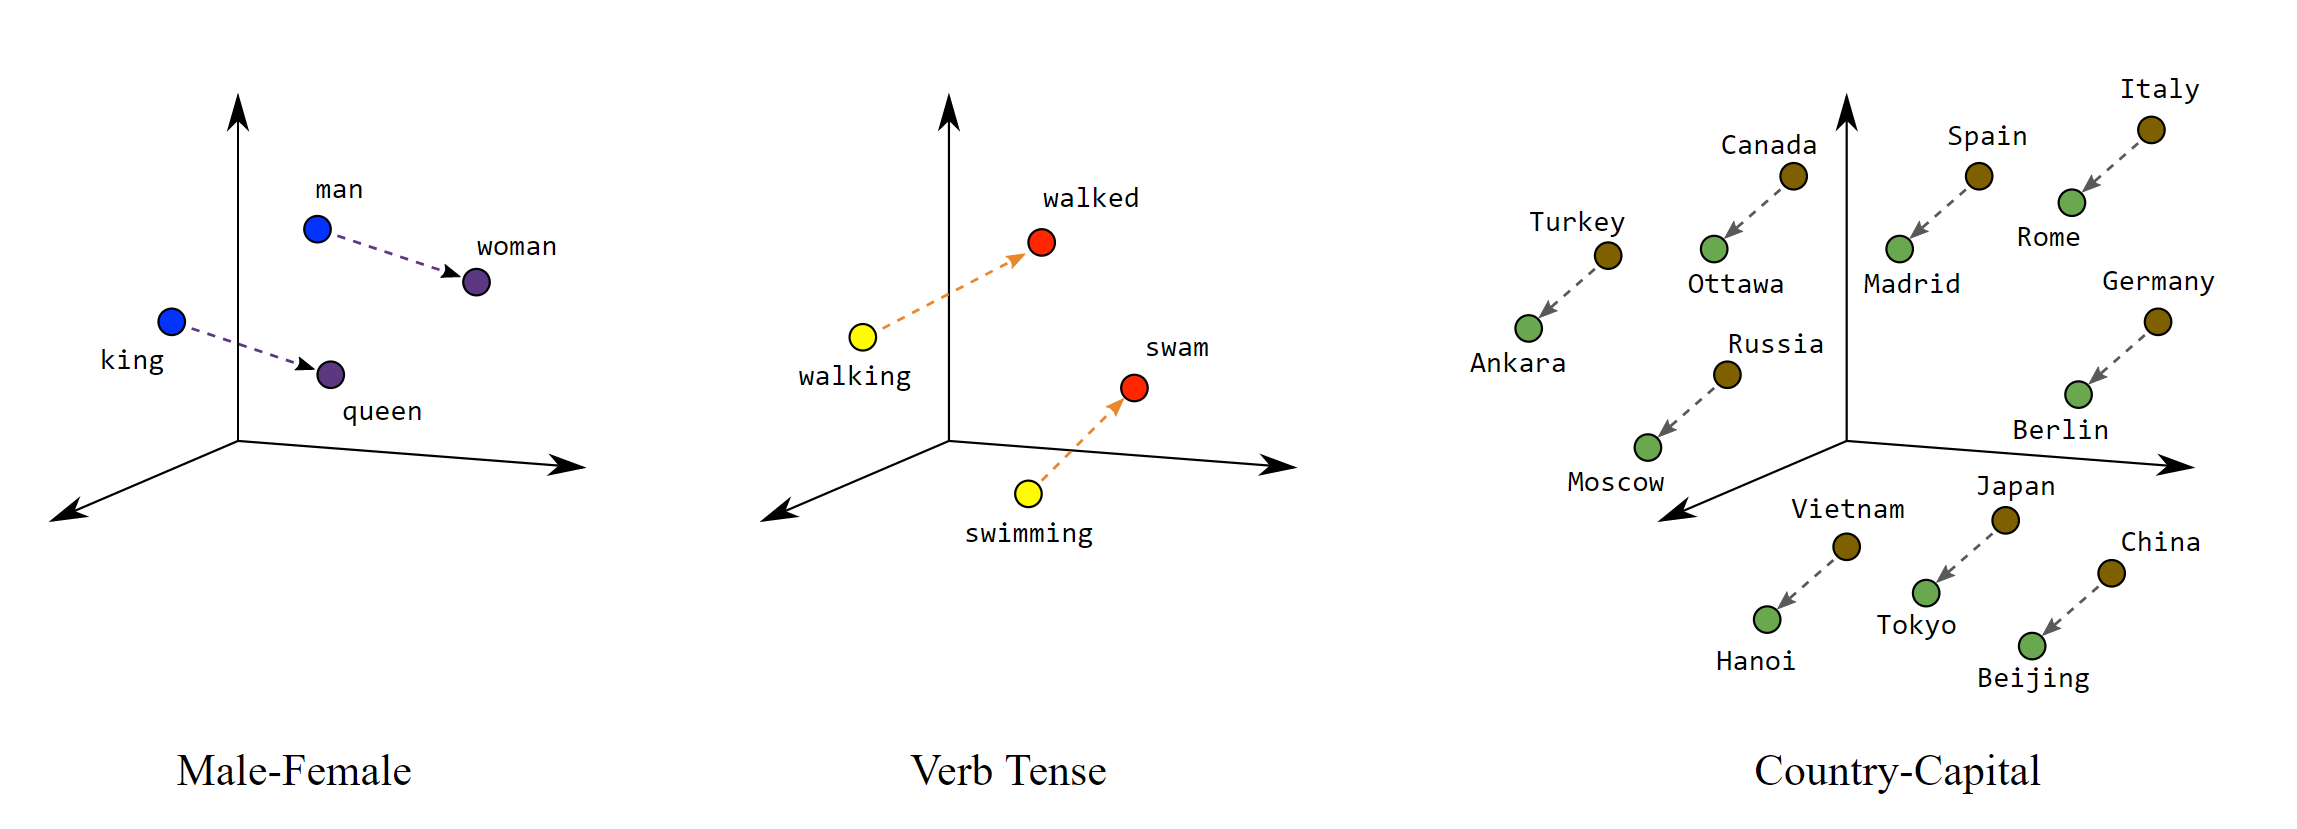
\includegraphics[width = 11cm]{figure/linear-relationships.png}\\ 
	\beamergotobutton{\href{https://developers.google.com/machine-learning/crash-course/embeddings/translating-to-a-lower-dimensional-space}{Source: Google}}
\end{figure}

\vfill
	
\end{frame}

% ------------------------------------------------------------------------------

\begin{frame}{embedding}
	
\vfill

\textbf{Document retrieval}

\begin{figure}
	\centering
		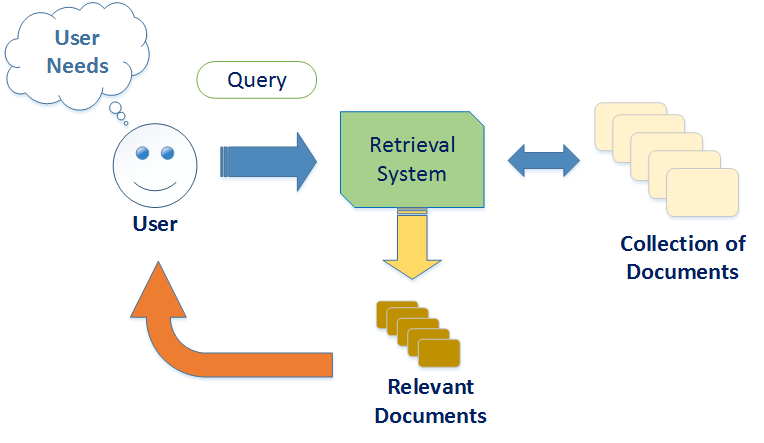
\includegraphics[width = 9cm]{figure/retrieval.png}\\ 
	\beamergotobutton{\href{https://www.analyticsvidhya.com/blog/2022/02/search-engines-using-deep-learning/}{Source: Analytics Vidhya}}
\end{figure}

\vfill

	
\end{frame}

% ------------------------------------------------------------------------------

\begin{frame}{pre-train/fine-tune}

\vfill

\textbf{Problem statement}

\begin{itemize}
	\item The larger the models, the more data is needed to train them
	\item (Labeled) Data is scarce and expensive!
	\item Many languages in the world are highly underrepresented in terms of existing resources\\
				Often: \textit{Number of speakers} $\neq$ \textit{Amount of available written text}
	\item Unlabeled (English) text data is ubiquitous
\end{itemize}
	
\vfill

\end{frame}

% ------------------------------------------------------------------------------

\begin{frame}{pre-train/fine-tune}

\vfill

\begin{figure}
	\centering
		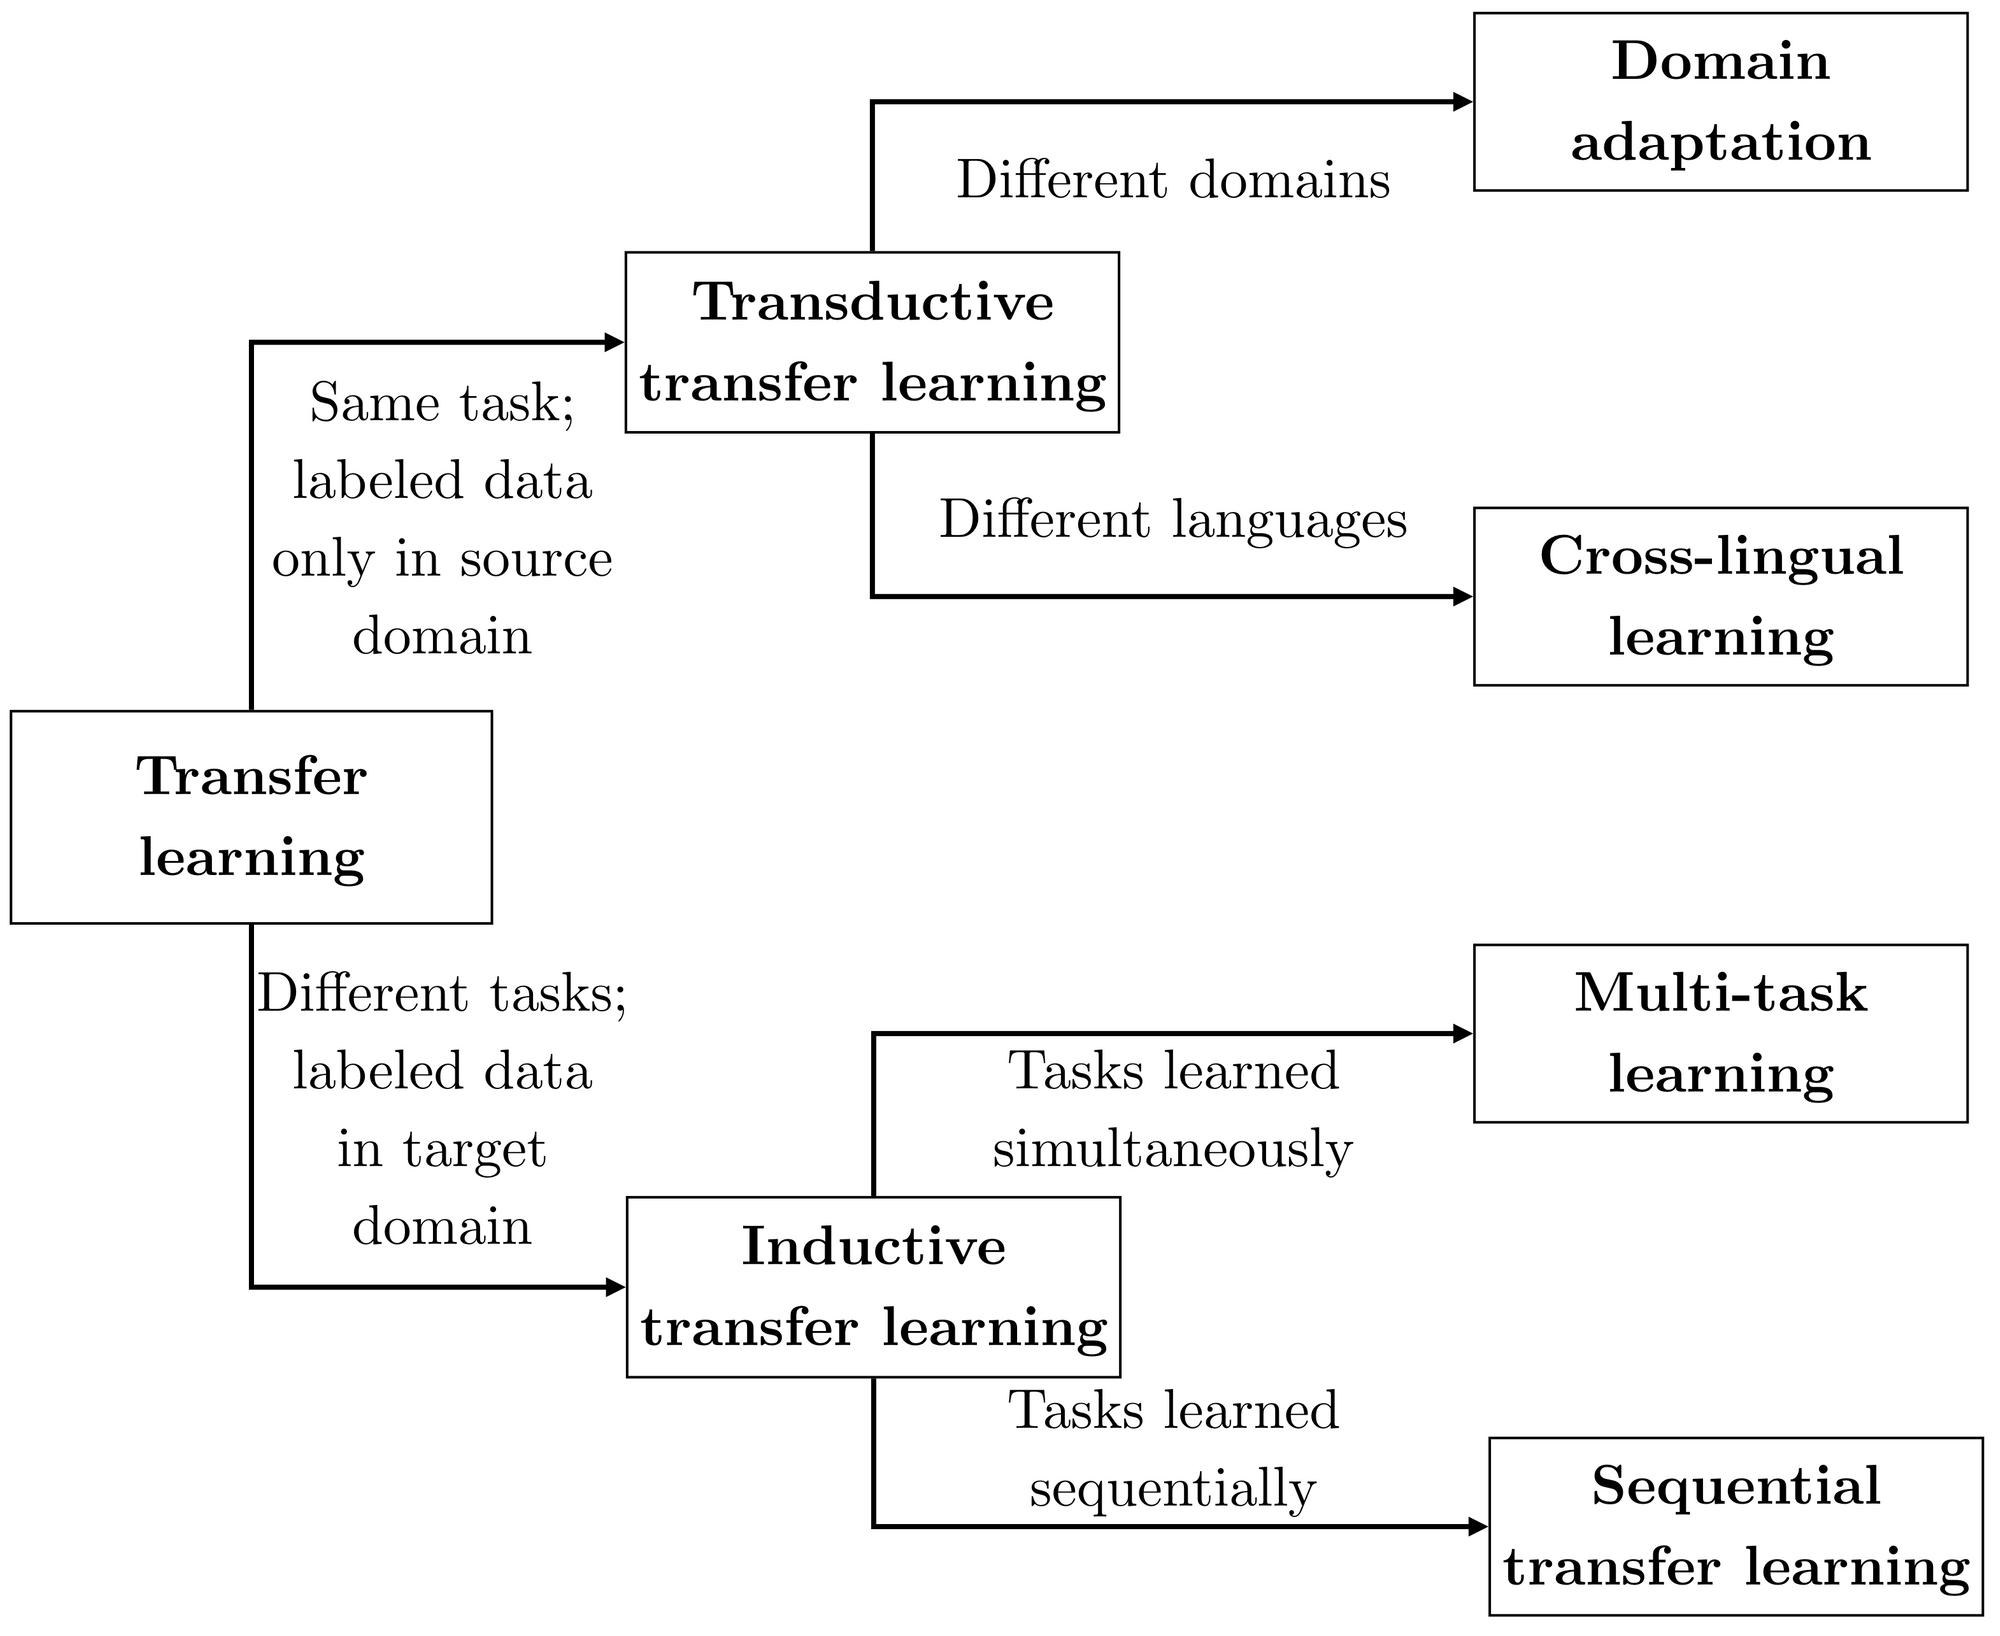
\includegraphics[width = 7cm]{figure/transfer_learning_taxonomy-1.png}\\ 
	\beamergotobutton{Taxonomy of transfer learning \href{https://ruder.io/thesis/}{(Source: Ruder, 2019)}}
\end{figure}

\vfill

\end{frame}

% ------------------------------------------------------------------------------

\begin{vbframe}{pre-train/fine-tune}

\vfill

\textbf{Pre-training:}

	\begin{itemize}
		\item Using unlabeled corpora in conjunction with self-supervised objectives 
					is commonly referred to as \textit{Pre-Training} the model
		\item Generation of samples for pre-training basically effortless, exploiting 
					the inherent structure of the text
		\item Construction of different self-supervised objectives, which are assumed
			\begin{itemize}
				\item to cover different phenomena better than the others
				\item to work more efficiently for learning
			\end{itemize}
	\end{itemize}
	
\vfill

\end{vbframe}

% ------------------------------------------------------------------------------

\begin{vbframe}{pre-train/fine-tune}

\vfill

\textbf{Fine-tuning:}

	\begin{itemize}
		\item The second phase of transfer learning, i.e. adapting the pre-trained model
					to a labeled data set for a specific downstream task is referred to as \textit{Fine-Tuning}
		\item Far less labeled data required compared to a scenario w/o pre-training
	\end{itemize}
	
\vfill

\end{vbframe}

% ------------------------------------------------------------------------------

\begin{vbframe}{prompting}

\vfill

\textbf{Accessing pre-trained models:}

	\begin{itemize}
		\item Fine-tune them
		\item Also possible: No fine-tuning, but .. 
			\begin{itemize}
				\item \textit{Zero-Shot Transfer} w/o ANY labeled data
				\item \textit{Few-Shot Transfer} w/ FEW labeled data points
			\end{itemize}
		\item In both of the latter cases, good pre-training becomes even more important
	\end{itemize}
	
\vfill

\end{vbframe}

% ------------------------------------------------------------------------------

\begin{vbframe}{prompting}

\vfill

\textbf{Definition(s):}

	\begin{itemize}
		\item \textit{GPT-3 paper:}\\ "Task Description" (accompanied by samples + labels)
		\item \textit{Prompt:} Describing the task the model is expected to perform
		\item \textit{Prompt Engineering:}\\ Finding the best prompt(s) for one (or across multiple) task(s)
		\item \textit{Prompt Tuning:}\\ Add trainable weights ("soft prompt") to inputs and fine-tune
	\end{itemize}
	
\vfill

\end{vbframe}

% ------------------------------------------------------------------------------

\begin{vbframe}{prompting}

\vfill
	
\textbf{Differences:}

\begin{figure}
	\centering
		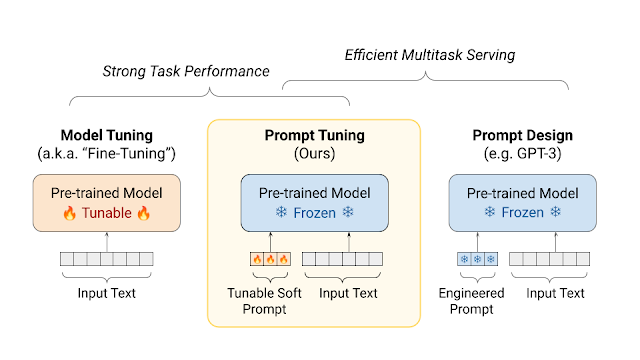
\includegraphics[width = 9cm]{figure/prompts.png}\\ 
	\beamergotobutton{\href{https://ai.googleblog.com/2022/02/guiding-frozen-language-models-with.html}{Source: Google}}
\end{figure}

\vfill

\end{vbframe}

% ------------------------------------------------------------------------------

\begin{vbframe}{chatting / generation}

\vfill
	
\textbf{Interacting with the model}

\begin{itemize}
	\item Larger model sizes, reduced latency and improved training regimes enable conversations with the models
	\item Enables the user to .. \\
	- .. have multi-turn conversations, with the model "remembering" previous inputs\\
	- .. refine the prompt in case of unsatisfactory output\\
	- .. used increased context sizes for the prompts
	\item Still: Static, pre-trained model with with "knowledge" 
\end{itemize}

\vfill

\end{vbframe}

% ------------------------------------------------------------------------------

\begin{vbframe}{chatting / generation}

\vfill
	
\textbf{Interacting with the model}

\begin{figure}
	\centering
		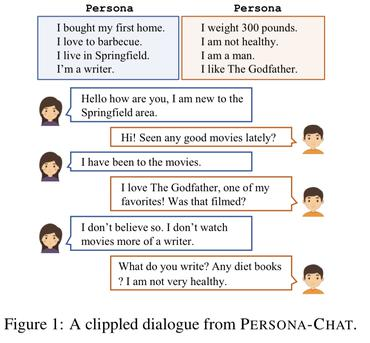
\includegraphics[width = 5cm]{figure/persona-chat.jpg}\\ 
	\beamergotobutton{\href{https://paperswithcode.com/task/code-generation}{Source: Papers with code (example for \texttt{Persona-Chat}}}
\end{figure}

\vfill

\end{vbframe}

% ------------------------------------------------------------------------------

\begin{vbframe}{chatting / generation}

\vfill
	
\textbf{Code generation}

\begin{figure}
	\centering
		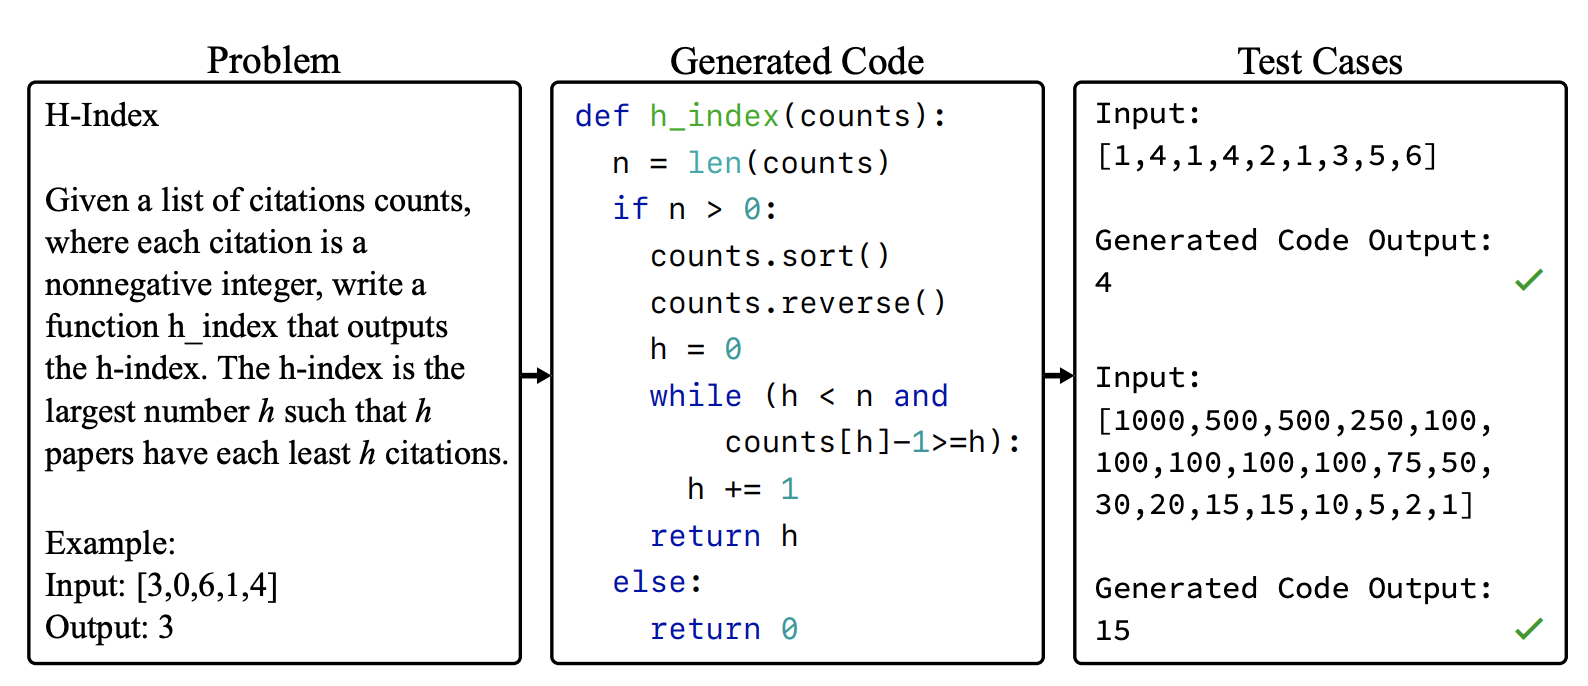
\includegraphics[width = 9cm]{figure/code-generation.png}\\ 
	\beamergotobutton{\href{https://paperswithcode.com/task/code-generation}{Source: Papers with code}}
\end{figure}

\vfill

\end{vbframe}

% ------------------------------------------------------------------------------

\begin{vbframe}{chatting / generation}

\vfill
	
\textbf{(Multi-)Document summarization}

\begin{figure}
	\centering
		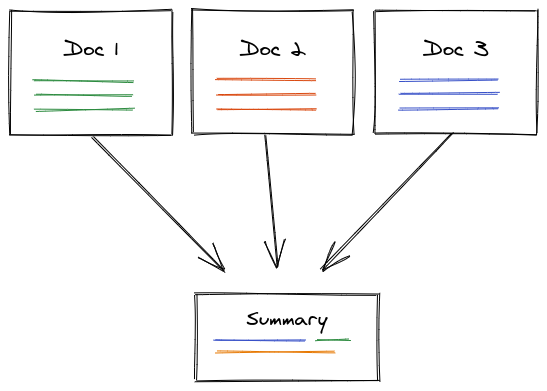
\includegraphics[width = 7cm]{figure/mds-diagram.png}\\ 
	\beamergotobutton{\href{https://aylien.com/blog/multi-document-summarisation-and-the-wcep-dataset}{Source: Aylien}}
\end{figure}

\vfill

\end{vbframe}

% ------------------------------------------------------------------------------

\begin{vbframe}{Outlook}

\vfill

\textbf{Agents}

	\begin{itemize}
		\item \textit{Example:} \href{https://python.langchain.com/docs/get_started/introduction.html}{LangChain}
		\item \textit{Goal:} The agent is able to solve complex task using tools and/or accessing the internet 
	\end{itemize}
	
\vfill

\end{vbframe}

% ------------------------------------------------------------------------------

\endlecture
\end{document}